\chapter{Análise dos resultados}
\label{cap:analise_resultados}
O presente Capítulo tem o objetivo de fazer a análise dos resultados obtidos por cada aplicação do \textit{benchmark} disponibilizado pelo NAS nas comparações das políticas de encaminhamento de fluxo.
A seção \ref{sec:aprentacao_dados} contém o necessário para a análise dos gráficos em relação às aplicações executadas. As demais Seções de \ref{sec:bt} até \ref{sec:sp} fazem a apresentação dos resultados individuais obtidos por cada aplicação do NAS. A Seção \ref{sec:consideracao_parcial} discute as diferenças e similaridades existentes nas políticas segundo os resultados obtidos.

\section{Apresentação dos Dados}
\label{sec:aprentacao_dados}

Os gráficos das seções \ref{sec:bt} a \ref{sec:sp} são representados da seguinte forma: cada gráfico é um programa do \emph{NAS} que executou um \emph{slots} MPI por computador da \emph{Fat Tree}, totalizando 16 \emph{slots}, ou seja, 16 processos. Foram feitas 10 execuções de cada aplicação do NAS por política, dessa forma foi obtido o tempo de execução para elaboração dos gráficos das Seções \ref{sec:bt} à \ref{sec:sp}. O eixo vertical representa o tempo em segundos que o programa levou para concluir a tarefa, este eixo foi deslocado da origem para facilitar a observação. No eixo horizontal estão as políticas de encaminhamento de fluxo. 

O CMT em laranja é a política que considera o consumo da largura de banda para encontrar o caminho de menor tráfego explicado na seção \ref{sec:bw}. Em azul, CMCP é a política de encaminhamento proativa que utiliza o caminho mais curto detalhado na Seção \ref{sec:pf}. Em amarelo os intervalos de tempo levados pela aplicação com a política CMCR, que utiliza o caminho mais curto reativamente explicado na Seção \ref{sec:rf}. Por último, o RR em verde é a política de \emph{round-robin} detalhado na Seção \ref{sec:rr}.

Cada elemento do gráfico em ordem crescente contém: valor mínimo representado pelo início do traço vertical inferior; primeiro quartil (25\% da amostra); segundo quartil representa os 50\% (mediana); terceiro quartil (75\% da amostra) e o fim do traço superior representa o maior tempo realizado. Os retângulos coloridos apresentam 50\% do conjunto de dados entre o primeiro e o terceiro quartil. Os intervalos entre mínimos e primeiro quartil contém 25\% da amostra assim como nos intervalos entre o terceiro quartil e o máximo.

\section{\textit{Block-Tridiagonal}}
\label{sec:bt}
\begin{figure}[!htb]
	\caption{\label{fig:bt}Tempo de execução da aplicação BT.}
	\begin{center}
	    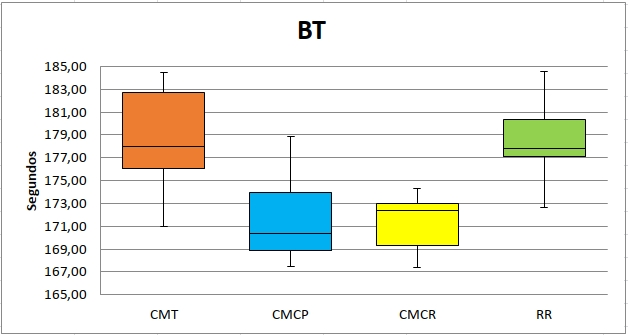
\includegraphics[scale=0.60]{imagens/bt.jpg}
	\end{center}
	\fonte{Elaborada pelo autor (2021).}	
\end{figure}
A aplicação BT, é um algoritmo de \textit{Gauss} para sistemas tridiagonal de blocos. 
O gráfico ilustrado na Figura \ref{fig:bt} representa a execução do programa para as políticas apresentadas. Começando pela política CMT, o menor tempo obtido foi de 171 segundos com um primeiro quartil de 176,11~s e uma mediana de 178,02~s. O terceiro quartil representando o 75\% da amostra foi de 182,76~s enquanto o maior tempo obtido por esta política foi 184,48~s. A  política CMCP teve o menor tempo em 167,51~s com um primeiro quartil de 168,86~s, mediana de 170,41~s e intervalo de 50\% dos valores da amostra fechou em 173,94~s no terceiro quartil. O maior tempo obtido por esta política foi 178,89~s.

A política de CMCR teve o menor tempo em 167 segundos como a política proativa. O tempo do primeiro quartil foi de 169~s, mediana de 172,35~s e terceiro quartil de 173,03~s. O intervalo de 50\% e o terceiro quartil apresentaram pouca variação de tempo sendo o maior tempo de execução dessa política foi de 174,34~s. A política de RR teve o menor tempo atingido em 172,64~s, com o primeiro quartil de 177,10~s, mediana de 177,86~s e terceiro quartil de 180,39~s. O maior tempo obtido nessa política foi 184,53~s.

Para os testes da aplicação BT, a política de CMCP apresentou a menor mediana de tempo seguido pela sua variante reativa CMCR, as políticas que atingiram maiores tempos são as que utilizam caminhos alternativos. A aplicação BT cria um total de 1070 fluxos transmitindo aproximadamente 48~MB durante seu processamento, a baixa comunicação faz com que as políticas que consideram o menor caminho CMCP e CMCR tenham melhores desempenhos por selecionarem caminhos com menos saltos, já que a quantidade de tráfego não é suficiente para gerar atrasos nos enlaces.  



\section{\textit{Conjugate Gradient}}
\label{sec:cg}

\begin{figure}[!htb]
	\caption{\label{fig:cg}Tempo de execução da aplicação CG.}
	\begin{center}
	    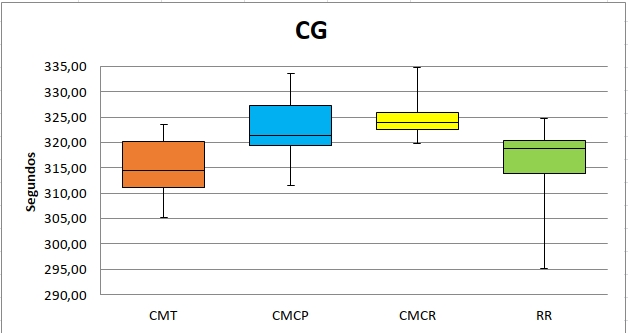
\includegraphics[scale=0.60]{imagens/cg.jpg}
	\end{center}
	\fonte{Elaborada pelo autor (2021).}	
\end{figure}
A aplicação de Gradiente Conjugado (CG) possui alta taxa de transferência de pacotes entre os 16 servidores, o tempo de execução é ilustrado pela Figura \ref{fig:cg}. A política CMT teve o menor valor de tempo obtido em 305,17~s com o primeiro quartil de 311,10~s, mediana de 314,45~s e terceiro quartil aproximado de 320,28~s. O maior valor obtido nas 10 execuções da aplicação BT para esta política foi de 323,56~s. Para a política CMCP o menor valor de tempo foi de 311,53~s, primeiro quartil de 319,44~s, mediana de 321,48~s e seu terceiro quartil de 327,28~s. O maior valor tempo atingido foi de 333,61 segundos. A política reativa CMCR apresentou o menor valor de 319,90~s com um primeiro quartil de 322,59~s, sua mediana foi de 323,88~s com um terceiro quartil de 325,83~s. O maior tempo que essa política levou para concluir BT foi 334,75~s. A política de RR apresentou o tempo mínimo em 295,07~s e primeiro quartil de 313,93~s, mediana de 318,79~s e o terceiro quartil de 320,48~s. O maior resultado de tempo~obtido~ foi 324,75~s. 

Dentre as políticas CMT obteve a menor mediana (314,45~s) seguido pela política RR, ambas apresentaram tempos menores em relação a variantes do caminho mais curto CMCP e CMCR. A aplicação CG cria 812 fluxos pelos quais são trafegados 101~MB, devido à alta taxa de transferência é possível notar uma queda na vantagem dos caminhos mais curtos com o aumento de tráfego. Em \cite{zhang2015performance}, em que o autor compara o desempenho do protocolo OSPF com a política fluxo CMCP de SDN, este comportamento também é observado com o aumento de fluxos, sendo que OSPF tem o desempenho melhor ao CMCP com pouco tráfego, e pior ao CMCP com o aumento do tráfego.



\section{\textit{Embarrassingly Parallel}}
\label{sec:ep}
\begin{figure}[!htb]
	\caption{\label{fig:ep}Tempo de execução da aplicação EP.}
	\begin{center}
	    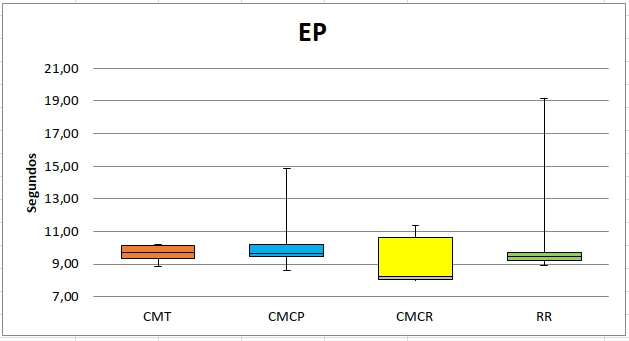
\includegraphics[scale=0.60]{imagens/ep.jpg}
	\end{center}
	\fonte{Elaborada pelo autor (2021).}	
\end{figure}
A aplicação de teste EP é um programa paralelo com pouca troca de informação entre os processos. Ilustrado pela Figura \ref{fig:ep} necessita transmitir aproximadamente 10~KB para a realização da tarefa ~\cite{marcondes2016executing}. Executando essa aplicação com a política CMT foi obtido um mínimo de 8,84~s, primeiro quartil de 9,33~s e uma mediana de 9,70~s. A variação de tempo nesta política foi mínima com o terceiro quartil fechando os 50\% do valor da amostra em 10,13~s e um máximo de 10,22~s. Para política de CMCP o mínimo obtido foi de 8,62~s, primeiro quartil e a mediana possuíram valores bem próximos sendo o primeiro de 9,46~s enquanto a mediana 9,66~s. O terceiro quartil foi de 10,20~s e o maior valor obtido de 14,88~s. A política de CMCR apresentou um mínimo de 7,95~s, primeiro quartil 8,04~s, mediana de 8,22~s e o terceiro quartil de 10,61~s. O máximo obtido foi de 11,35~s. Para a política de RR  foi obtido um mínimo de 8,93~s, primeiro quartil que representa 25\% dos valores apresentou 9,21~s e mediana de 9,49~s. O terceiro quartil representando os 75\% dos valores foi de 9,69~s e o maior tempo de 19,15~s, sendo o que atingiu o maior máximo. 

A aplicação EP cria 714 fluxos pelos quais são transferidos 10 KB durante seu tempo de execução, a baixa variação de tempo representado no gráfico sugere que com pouca informação trafegada não há diferença visível entre as políticas, ainda assim, o esperado seria de que as políticas de caminho mais curto CMCP e CMCR tivessem maior vantagem, conforme mencionado na Seção \ref{sec:bt} e \ref{sec:cg}. A variação de RR ocorre devido à escolha de rotas com muitas quantidades de saltos, é possível notar que os 75\% da amostra dessa política tiveram variações entre 9 e 10 segundos.

\section{\textit{Integer sort}}
\label{sec:is}
\begin{figure}[!htb]
	\caption{\label{fig:is}Tempo de execução da aplicação IS.}
	\begin{center}
	    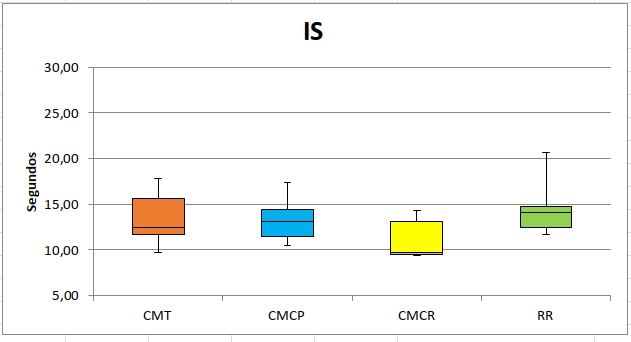
\includegraphics[scale=0.60]{imagens/is.jpg}
	\end{center}
	\fonte{Elaborada pelo autor (2021).}	
\end{figure}

O programa IS assim como BT e EP fazem pouca troca de informação em relação as demais, durante sua execução são criados 2384 fluxos, o objetivo desse programa é fazer a ordenação de números inteiros de forma paralela. Representando pela Figura \ref{fig:is}, o menor valor obtido pela política CMT é 9,75~s, primeiro quartil de 11,73~s e mediana de 12,41~s. O terceiro quartil é de 15,65~s e o valor de tempo máximo obtido para esta política foi de 17,83~s. Para política CMCP o tempo mínimo foi de 10,45~s, primeiro quartil de 11,45~s e mediana de 13,11~s, o terceiro quartil foi de 14,38~s e o maior tempo obtido nesta política foi de 17,37 segundos. A política de CMCR teve o valor mínimo de 9,43~s bem próximo ao primeiro quartil de 9,46~s e mediana de 9,69~s. O terceiro quartil foi de 13,17~s e 14,32~s. A política de RR teve seu menor tempo de execução em 11,65~s. Seu primeiro quartil 12,47~s e mediana em 14,07~s fechando o intervalo de 75\% dos valores com o terceiro quartil em 14,80~s.  O maior tempo de execução obtido por esta política na realização da tarefa foi 20,62 segundos. Observando o gráfico é possível perceber que não existe diferença entre as políticas em relação ao desempenho da aplicação IS. 

\section{\textit{Lower Upper}}
\label{sec:lu}
\begin{figure}[!htb]
	\caption{\label{fig:lu}Tempo de execução da aplicação LU.}
	\begin{center}
	    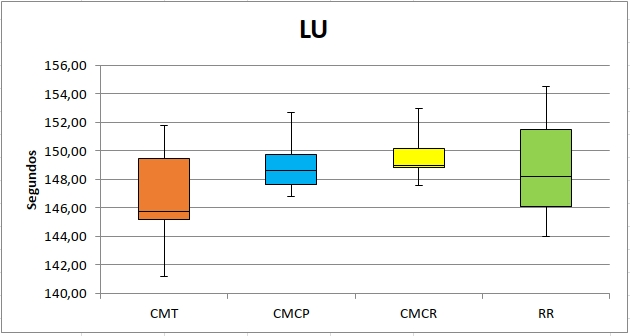
\includegraphics[scale=0.60]{imagens/lu.jpg}
	\end{center}
	\fonte{Elaborada pelo autor (2021).}	
\end{figure}
A Figura \ref{fig:lu} representa os tempos te execução da aplicação \textit{Lower-Upper Gauss-Seidel solver} (LU). A política CMT teve o menor tempo de 141,18~s, primeiro quartil de 145,17~s próximo da mediana de 145,72~s. O terceiro quartil de 149,45~s e o máximo obtido nessa política foi de 151,78~s. Para a política de CMCP o mínimo foi de 146,81~s e o primeiro quartil de 147,68~s, a mediana foi de 148,61~s e terceiro quartil representando os 75\% dos valores foi de 149,76~s. O máximo atingido por essa política de 152,72~s.  
Para a política de CMCR o menor tempo foi de 147,57~s. O primeiro quartil de 148,85~s, mediana de 148,94~s e terceiro quartil de 150,17~s. O maior tempo atingido foi de 152,95~s. A política de RR teve o menor tempo de 143,98~s, primeiro quartil de 146,09~s e mediana de 148,18~s. O terceiro quartil foi de 151,48~s, o maior tempo obtido de 154,54~s. 

A menor mediana foi da política de CMT, que também apresentou o menor tempo de execução. Em 820 fluxos criados foram transferidos entre os servidores 496,80~MB durante o tempo de execução, as políticas de rotas alternativas CMT e RR apresentaram tempos menores que os algoritmos de caminho mais curto. Conforme mencionado em \ref{sec:cg} o aumento de tráfego dos enlaces começam a gerar atrasos nas políticas que utilizam o caminho mais curto.


\section{\textit{Multigrid}}

\label{sec:mg}
\begin{figure}[!htb]
	\caption{\label{fig:mg}Tempo de execução da aplicação MG.}
	\begin{center}
	    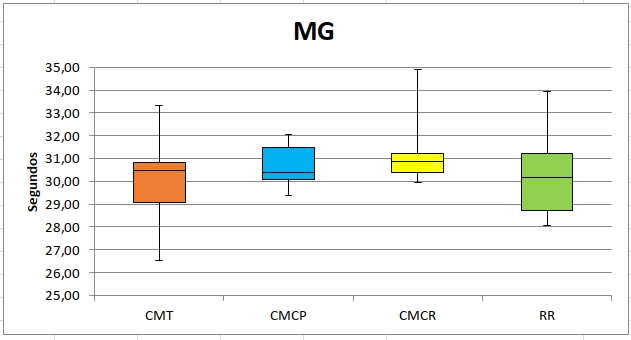
\includegraphics[scale=0.60]{imagens/mg.jpg}
	\end{center}
	\fonte{Elaborada pelo autor (2021).}	
\end{figure}
A aplicação \textit{Multi-Grid} (MG)  possui um baixo tempo de execução com altas taxas de transferência de pacotes entre os serviços hospedados nos 16 servidores \cite{marcondes2016executing}. Para o teste do MG ilustrado na Figura \ref{fig:mg}, o menor tempo obtido pela política CMT foi 26,55~s. O primeiro quartil foi de 29,09~s e a mediana de 30,46~s próxima ao valor do terceiro quartil de 30,80~s. O maior valor obtido no intervalo de 10 execuções foi de 33,32~s. A política CMCP teve o menor valor obtido em 29,36~s, primeiro quartil de 30,06~s, mediana de 30,37~s e terceiro quartil de 31,46~s. O maior tempo de execução dessa política foi de 32,03~s. A política de CMCR teve seu menor tempo de 29,93~s, primeiro quartil de 30,38~s, mediana de 30,85~s e terceiro quartil de 31,22~s. O maior tempo no intervalo de 10 execuções foi de 34,89~s sendo também o maior tempo global de execução para esta aplicação. A política RR teve o menor tempo de 28,05~s, primeiro quartil de 28,73~s, mediana de 30,17~s e terceiro quartil de 31,23~s. O maior tempo obtido nessa política foi de 33,95 segundos. 

A aplicação MG tem um volume de dados trafegados na rede de 101.24~MB durante seus 30 segundos de execução, na qual são criados 838 fluxos. Observando o gráfico é possível notar que todas as políticas tiveram a mesma mediana (30~s). A troca de informações não é alta o suficiente para gerar gargalos na rede mas também não apresenta vantagens para rotas alternativas embora estas tenham conseguido obter 25\% dos valores de tempos menores que as CMCP e CMCR. 

\section{\textit{Solution Pentadiagonal}}
\label{sec:sp}
\begin{figure}[!htb]
	\caption{\label{fig:sp}Tempo de execução da aplicação SP.}
	\begin{center}
	    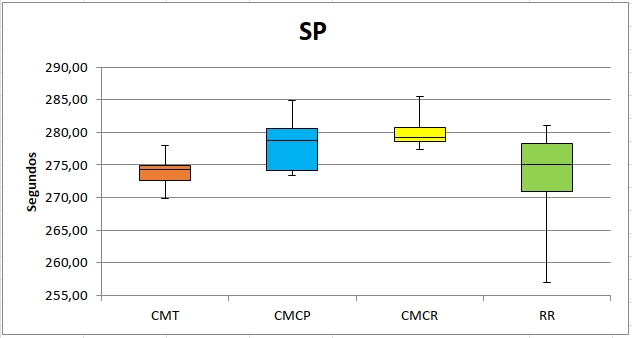
\includegraphics[scale=0.60]{imagens/sp.jpg}
	\end{center}
	\fonte{Elaborada pelo autor (2021).}	
\end{figure}
A aplicação SP do \textit{benchmark} NAS tem o maior volume de dados transferido durante a solução da tarefa, assim como uma das maiores taxas de transferências dentre todas as aplicações. A  Figura \ref{fig:sp} representa o tempo de execução dessa aplicação em relação das políticas. Para CMT o menor tempo foi de 269,78~s com o primeiro quartil de 272,59~s, mediana de 274,29~s e o terceiro quartil de 274,88~s. O maior tempo levado por essa aplicação foi 277,95 segundos. A política CMCP teve o menor tempo de 273,40 s, primeiro quartil de 274,16~s, mediana de 278,81~s e terceiro quartil de 280,61~s. O maior tempo foi de 284,92~s. 
A política de CMCR teve seu menor tempo em 277,36~s, primeiro quartil de 278,53~s, mediana de 279,26~s e terceiro quartil 280,76~s. O seu maior tempo foi de 285,50~s. Já a política de RR teve seu menor tempo de 256,91~s apresentando também o menor mínimo global. O primeiro quartil foi de 270,87~s, mediana de 275,06~s, terceiro quartil de 278,29~s e maior tempo obtido por esta política foi de 280,99 segundos.

Os tempos de execução apresentou a menor mediana com as políticas de CMT e RR em aproximadamente 174 segundos. A política que teve o menor mínimo apresentado foi o RR com 256 segundos. Os que tiveram maior máxima foram o CMCP e o CMCR, próximos a 180 segundos. Conforme as análises anteriores, já era esperado que para essa aplicação SP tivesse vantagem as políticas de múltiplos caminhos devido ao auto volume de dados transferidos, foram criados 1760 fluxos pelos quais foram transferidos um total de (1707~ MB). Sendo assim, quanto maior é a transferência mais visível é a diferença entre essas políticas.


\section{Discussão dos Resultados}
\label{sec:discussao_resultados}
 Em relação análise dos gráficos é possível perceber que aplicações com pouco volume de tráfego possui uma vantagem nas políticas que utilizam o caminho mais curto CMCP e CMCR (saltos), como é o caso das aplicações BT, EP e IS. Isso ocorre por não haver tráfego suficiente para causar sobrecarga ou atrasos nos enlaces, sendo assim, quanto menos saltos, menor a quantidade de comutadores processando tráfego, assim como escalonamento do processador. 

Em algumas aplicações do teste como  SP, MG e CG que necessitam maiores trocas de informações, as políticas que utilizam rotas alternativas obtiveram menores mínimos e a variação de 50\% da amostra representado ganho na mediana tempo de execução para políticas com rotas alternativas RR e CMT. Por exemplo, na aplicação CG  foi apontado pela mediana, cerca de 5 segundos de ganho em relação às políticas CMCP e CMCR ilustrado pela Figura \ref{fig:cg}. Os resultados demonstram que aplicações com pouco tráfego são favorecidas pesas políticas com menor quantidade de saltos mesmo que utilizem sempre as mesmas rotas, já nas aplicações com maiores tráfegos são favorecidas as políticas de rotas alternativas. Já entre as aplicações que ficam entre baixa e alta troca de informações os resultados são muito próximos entre si, não sendo visível a diferença.

Em relação à política CMT, o menor intervalo de tempo permitido pelo controlador na coleta de bits transmitidos necessários para os cálculos de vazão, são períodos de 1 segundo, o que pode ser considerado um tempo grande para medir fluxos que alternam de forma tão rápida. Autores que utilizaram dessa abordagem na construção de algorítimos com peso dos enlaces dinâmicos como é o caso de \cite{akin2019comparison} também encontraram desafios relacionados a consultas do plano de dados. Quando o controlador faz muitas requisições ao plano de dados, para obter estatísticas mais atualizadas é gerado excesso de tráfego na rede, mas se o controlador acessa em períodos maiores, a informação se tornam desatualizadas. Neste caso é considerado pesos que não refletem exatamente o estado atual da rede. A ainda soluções que propõem manter uma imagem do plano de dados no plano de controle. Assim quando um fluxo é criado ou removido pelo controlador é armazenado essa informação em um grafo. Dessa forma a quantidade de tráfego de um caminho é estimado pela quantidade de fluxos ativos que ele possui. Apesar desse método não necessitar consultar o plano de dados, a estimativa precisa não é uma tarefa fácil. Em \cite{singh2017estimation}, o autor propõe uma forma de estimar a largura de banda utilizada pelos fluxos através leituras periódicas, de modo a aproximar a imagem que o controlador tem do plano de dados.  

A política RR foi a que apresentou maior dispersão de tempo, como mostra as Figuras  \ref{fig:cg}, \ref{fig:ep} e \ref{fig:sp}. Essa dispersão ocorre devido à alternância de rotas considerar caminhos com muitos saltos desnecessários, assim como a possibilidade de escolha de caminhos que podem conter o tráfego elevado. 


\section{Considerações Parciais}
\label{sec:consideracao_parcial}
O presente Capítulo apresentou os resultados obtidos pelo \textit{benchmark} NAS, na quais são baseadas em resolução de problemas reais em sistemas de processamento paralelo. O Capítulo expressou em forma de gráficos \textit{bloxpot} as aplicações da ferramenta individualmente para cada política implementada, com o objetivo de realizar um estudo sobre o comportamento dessas aplicações em relação da forma como o encaminhamento de fluxo é feito. 

É possível notar que embora políticas que utilizam a menor quantidade de saltos para o encaminhamento sejam melhores com baixo volume de tráfego, essa vantagem vai sendo perdida a medida que o volume de tráfego vai aumentando, até que as rotas alternativas começam apresentar vantagem. Como é um ambiente emulado a quantidade de comutadores existentes no caminho influenciam na transferência de dados devido ao número de processos ativos, (\textit{e.g.}, controlador multi-thread, comutadores, ferramenta NAS), essa mudança pode ser visível com o aumento do número de saltos na política de RR causando mais variações. 